\documentclass[a4paper,14pt]{extarticle} 
\usepackage[a4paper,top=1.5cm, bottom=1.5cm, left=2cm, right=1cm]{geometry}
%\usepackage[T2A]{fontenc}
%\usepackage[english, russian]{babel}
\usepackage{graphicx}
\DeclareGraphicsExtensions{.pdf,.png,.jpg}
\usepackage{fontspec}
\setmainfont{Times New Roman}
\setsansfont{FreeSans}
\setmonofont{FreeMono}
\renewcommand{\baselinestretch}{1.5}
\usepackage{polyglossia}
\setdefaultlanguage{russian}
\setotherlanguages{english,russian}
\usepackage{setspace}
\usepackage[many]{tcolorbox}
\usepackage{listings}
\usepackage{multicol}
\usepackage{xcolor}
\usepackage{pdfpages}

\definecolor{codegreen}{rgb}{0,0.6,0}
\definecolor{codegray}{rgb}{0.5,0.5,0.5}
\definecolor{codepurple}{rgb}{0.58,0,0.82}
\definecolor{backcolour}{rgb}{0.95,0.95,0.92}

\lstdefinestyle{mystyle}{
    backgroundcolor=\color{backcolour},   
    keywordstyle=\color{magenta},
    numberstyle=\tiny\color{codegray},
    stringstyle=\color{codepurple},
    basicstyle=\ttfamily\footnotesize,
    breakatwhitespace=false,         
    breaklines=true,                 
    captionpos=b,                    
    keepspaces=true,                 
    numbers=left,                    
    numbersep=5pt,                  
    showspaces=false,                
    showstringspaces=false,
    showtabs=false,                  
    tabsize=2
}

\lstset{style=mystyle}

\begin{document}
    \begin{center}
        \thispagestyle{empty}
        \begin{singlespace}
        ФЕДЕРАЛЬНОЕ АГЕНТСТВО СВЯЗИ

        ФЕДЕРАЛЬНОЕ ГОСУДАРСТВЕННОЕ БЮДЖЕТНОЕ ОБРАЗОВАТЕЛЬНОЕ

        УЧРЕЖДЕНИЕ ВЫСШЕГО ОБРАЗОВАНИЯ

        «САНКТ-ПЕТЕРБУРГСКИЙ ГОСУДАРСТВЕННЫЙ УНИВЕРСИТЕТ ТЕЛЕКОММУНИКАЦИЙ ИМ. ПРОФ. М.А. БОНЧ-БРУЕВИЧА»

        (СПбГУТ)
        \end{singlespace}
        \vspace{-1ex}
        \rule{\textwidth}{0.4pt}
        \vspace{-5ex}

        Факультет \underline{Инфокоммуникационных сетей и систем}

        Кафедра \underline{Защищенных систем связи}
        \vspace{10ex}

        \textbf{Лабораторная работа №1}\\
        


    \end{center}
    \vspace{4ex}
    \begin{flushright}
    \parbox{10 cm}{
    \begin{flushleft}
        Выполнили студенты группы ИКТЗ-83:

        \underline{Громов А.А., Миколаени М.С., Мазеин Д.С.} \hfill \rule[-0.85ex]{0.1\textwidth}{0.6pt}

        \footnotesize \textit{ (Ф.И.О., № группы) \hfill (подпись)} \normalsize

        Проверил:

        \underline{Казанцев А.А.} \hfill \rule[-0.85ex]{0.1\textwidth}{0.6pt}

        (\footnotesize \textit{уч. степень, уч. звание, Ф.И.О.) \hfill (подпись)} \normalsize

    \end{flushleft}
    }
    \end{flushright}
    \begin{center}
        \vfill
        Санкт-Петербург

        2021

    \end{center}
    \newpage

    \textbf{Цель лабораторной работы:}

    \textbf{Пункт 1 - Ознакомьтесь с параметрами настройки политик МЭ.}
    \begin{center}
        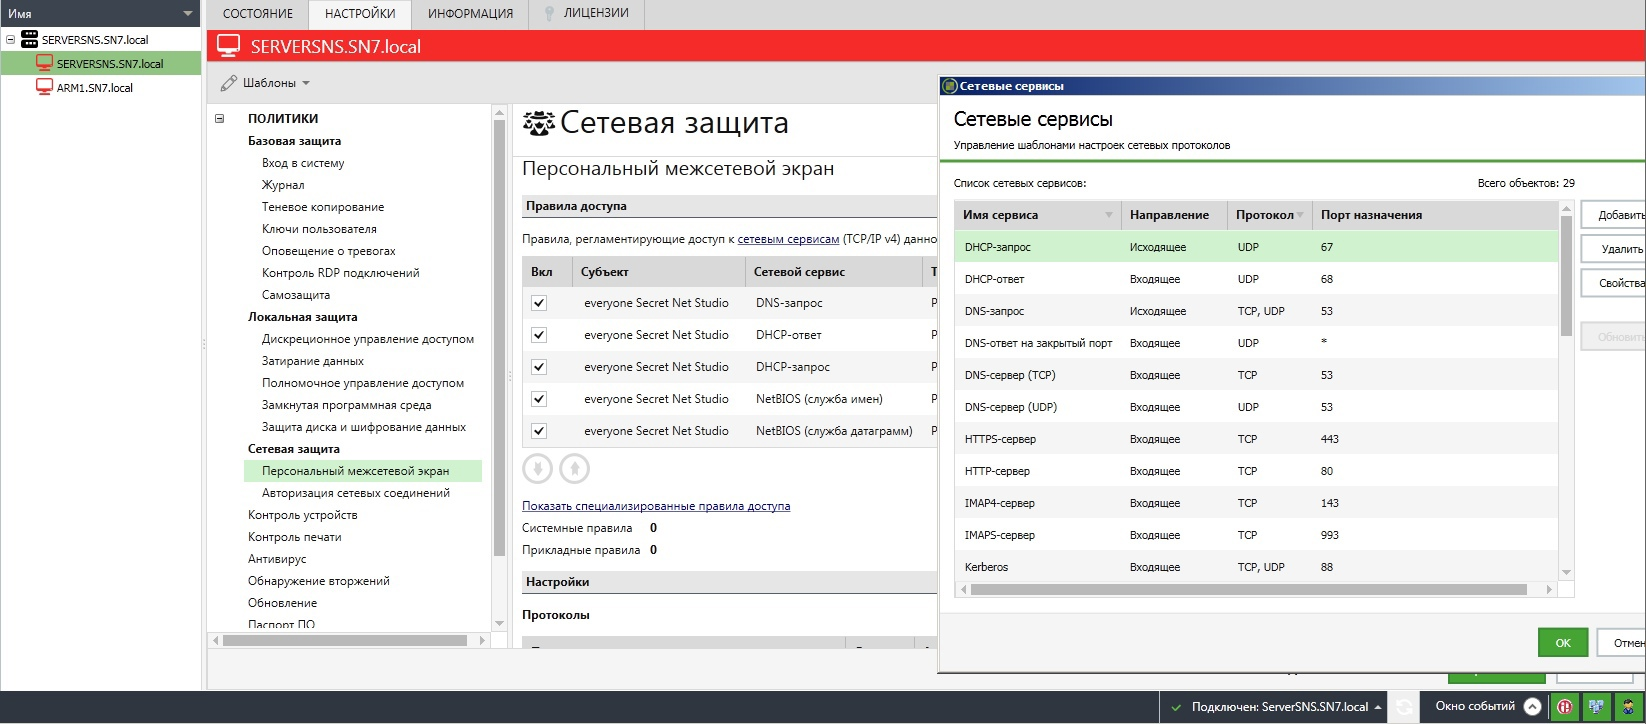
\includegraphics[scale=0.3]{pics/1.jpg}

       Настройки политик МЭ.
    \end{center}

    \textbf{Пункт 3 - Добавление нового сетевого сервиса для доступа к серверу IIS по порту 8090}
    \begin{center}
        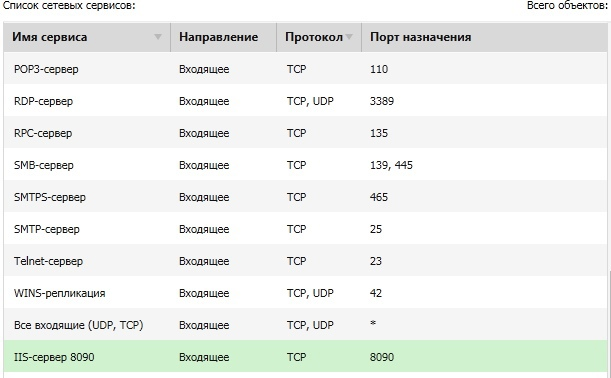
\includegraphics[scale=0.6]{pics/3.jpg}

       Список сетевых сервисов.
    \end{center}

    \newpage
    \textbf{Пункт 5 - Проверка доступа RDP-подключения}
    \begin{center}
        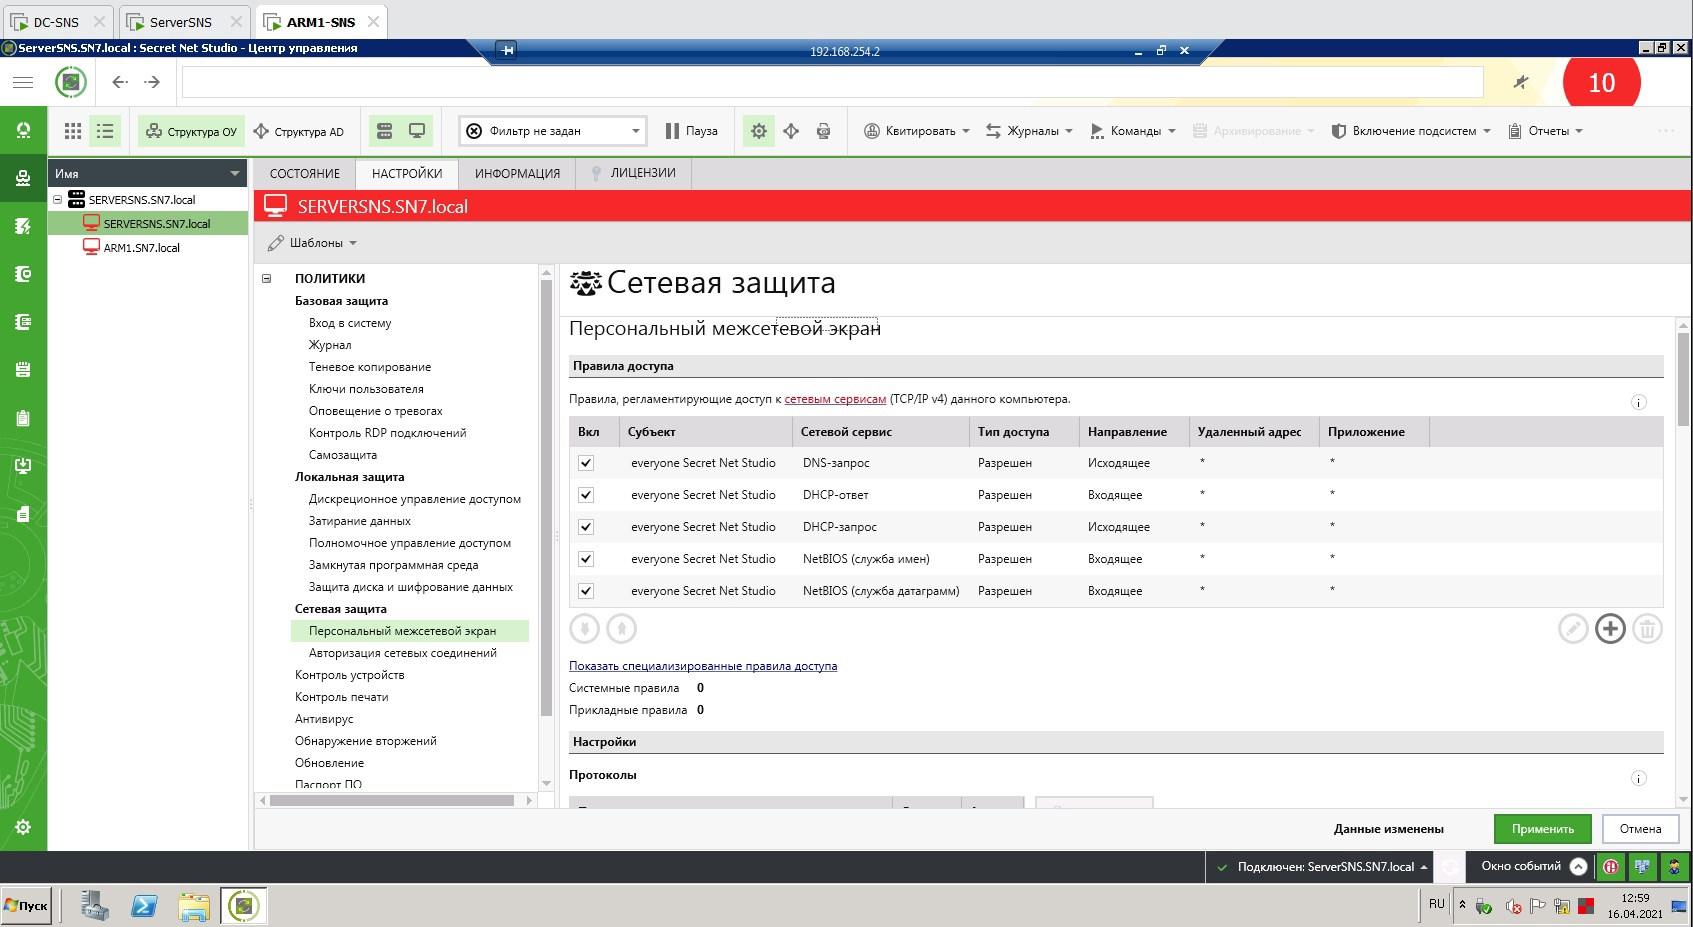
\includegraphics[scale=0.3]{pics/5.jpg}

        RDP-соединение.
    \end{center}

    \textbf{Пункт 13 - Создание правила запрета подключения по RDP к ServerSNS}
    \begin{center}
        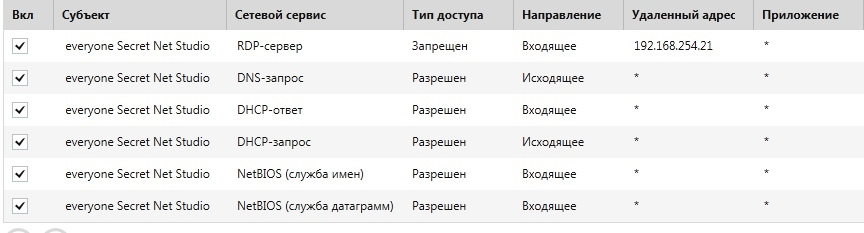
\includegraphics[scale=0.55]{pics/13.jpg}

       Список правил.
    \end{center}

    \textbf{Пункт 16 - Правила фильтрации доступа к сетевму сервису IIS-сервер 8090}
    \begin{center}
        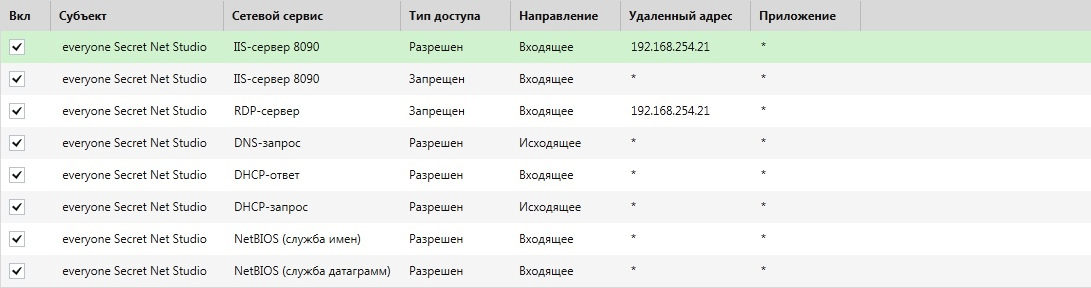
\includegraphics[scale=0.45]{pics/16.jpg}

       Список правил.
    \end{center}
    
    \textbf{Пункт 17 - Специализированные правила доступа }
    \begin{center}
        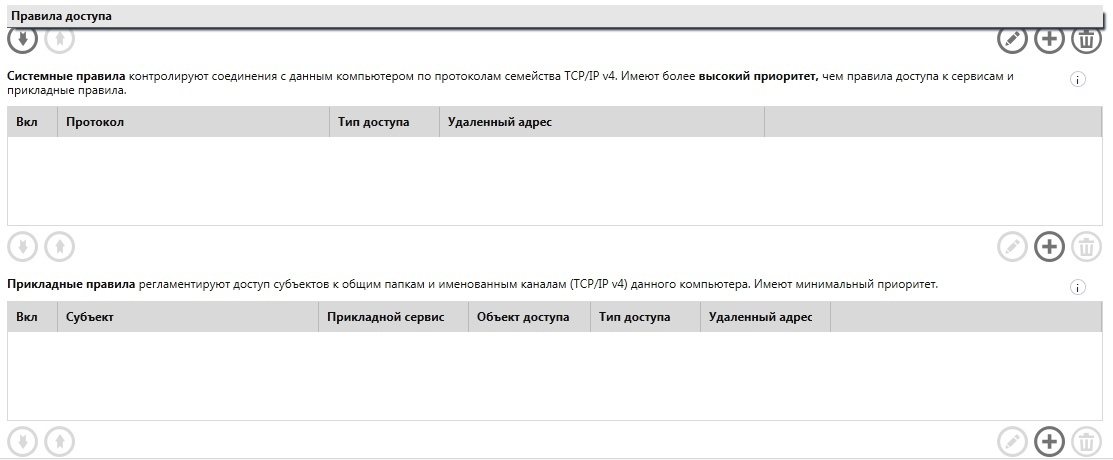
\includegraphics[scale=0.45]{pics/17.jpg}

        Специализированные правила доступа.
    \end{center}

    \textbf{Пункт 18 - Пример настройки запрета доступа к серверу ServerSNS по RDP-протоколу.}
    \begin{center}
        \begin{multicols}{2}
            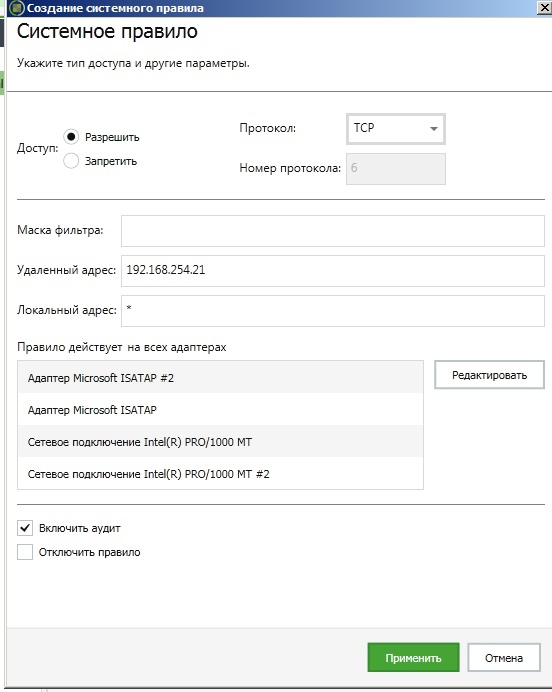
\includegraphics[scale=0.4]{pics/18_1.jpg}
            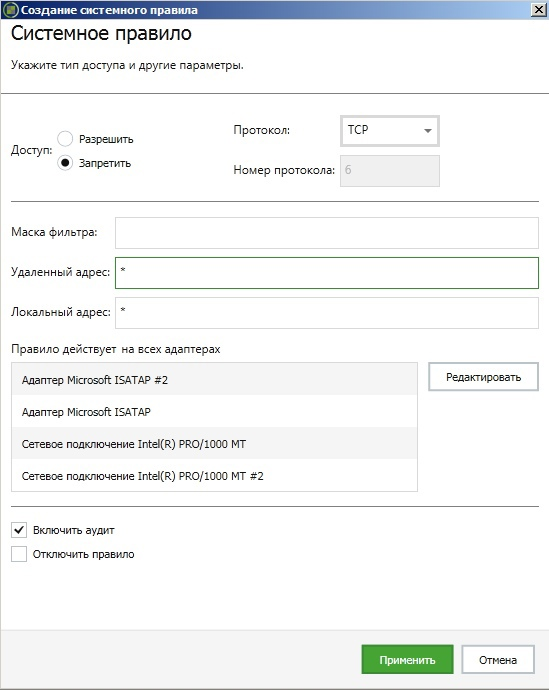
\includegraphics[scale=0.4]{pics/18_2.jpg}
        \end{multicols}

        Окно настройки правила.
    \end{center}

    \newpage
    \textbf{Пункт 19 - Создание прикладного правилa}
    \begin{center}
        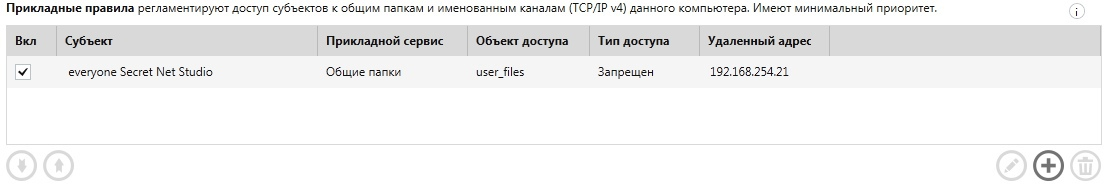
\includegraphics[scale=0.42]{pics/19_1.jpg}\\
        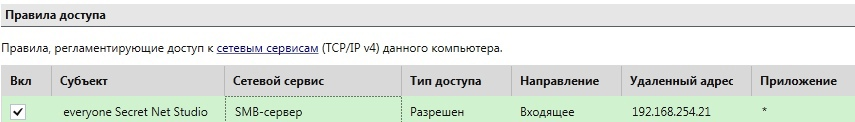
\includegraphics[scale=0.55]{pics/19_2.jpg}

        Прикладное правило.
    \end{center}
  
    \textbf{Пункт 23.1 - Проверка команды ping с выключенной ICMP защитой}
    \begin{center}
        \begin{multicols}{2}
            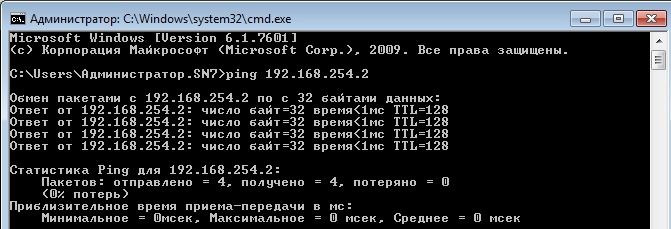
\includegraphics[scale=0.4]{pics/23.1_1.jpg}
            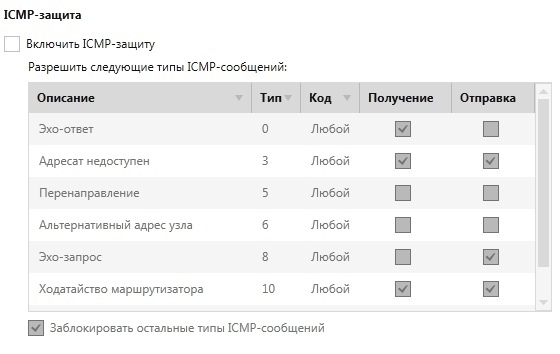
\includegraphics[scale=0.4]{pics/23.1_2.jpg}
        \end{multicols}

        Команда пинг и правила.
    \end{center}

    \textbf{Пункт 23.2 - Проверка команды ping с включенной ICMP защитой}
    \begin{center}
        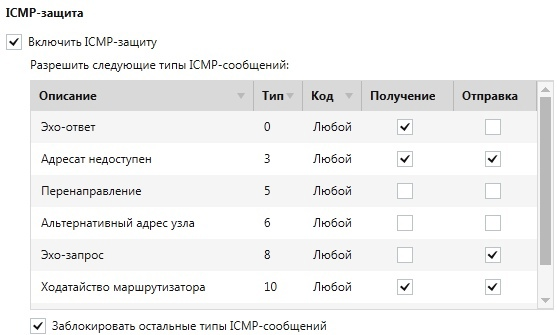
\includegraphics[scale=0.45]{pics/23.2_1.jpg}
        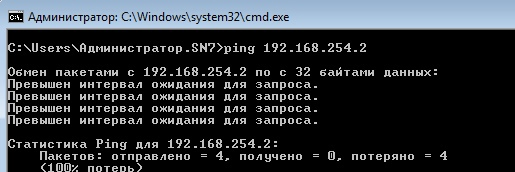
\includegraphics[scale=0.45]{pics/23.2_2.jpg}

        Команда пинг и правила.
    \end{center}

    \newpage
    \textbf{Пункт 24 - Тестирование работы правил}
    \begin{center}
        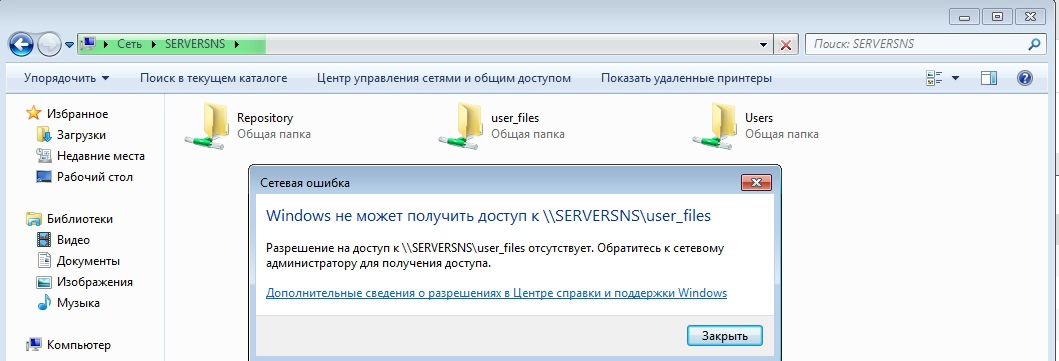
\includegraphics[scale=0.35]{pics/24_1.jpg}\\
        \vspace{2ex}
        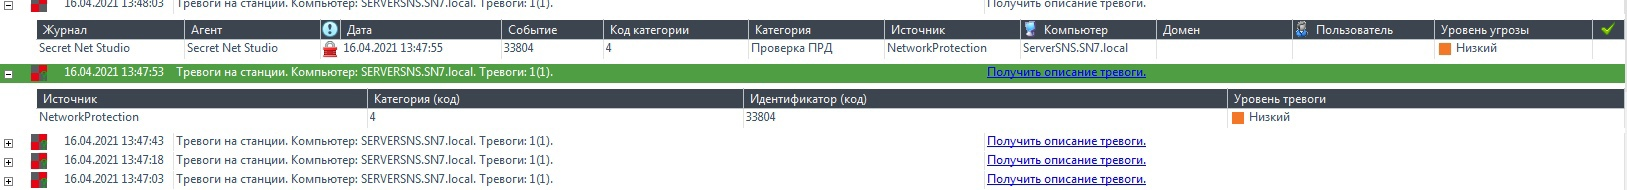
\includegraphics[scale=0.25]{pics/24_2.jpg}\\
        \vspace{2ex}
        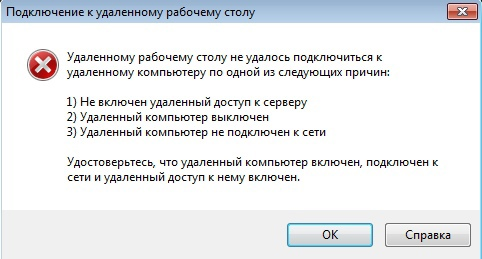
\includegraphics[scale=0.6]{pics/24_3.jpg}

        Работа правил.
    \end{center}
\end{document}

